\begin{figure*}[h]
\centering
% 6 examples
% 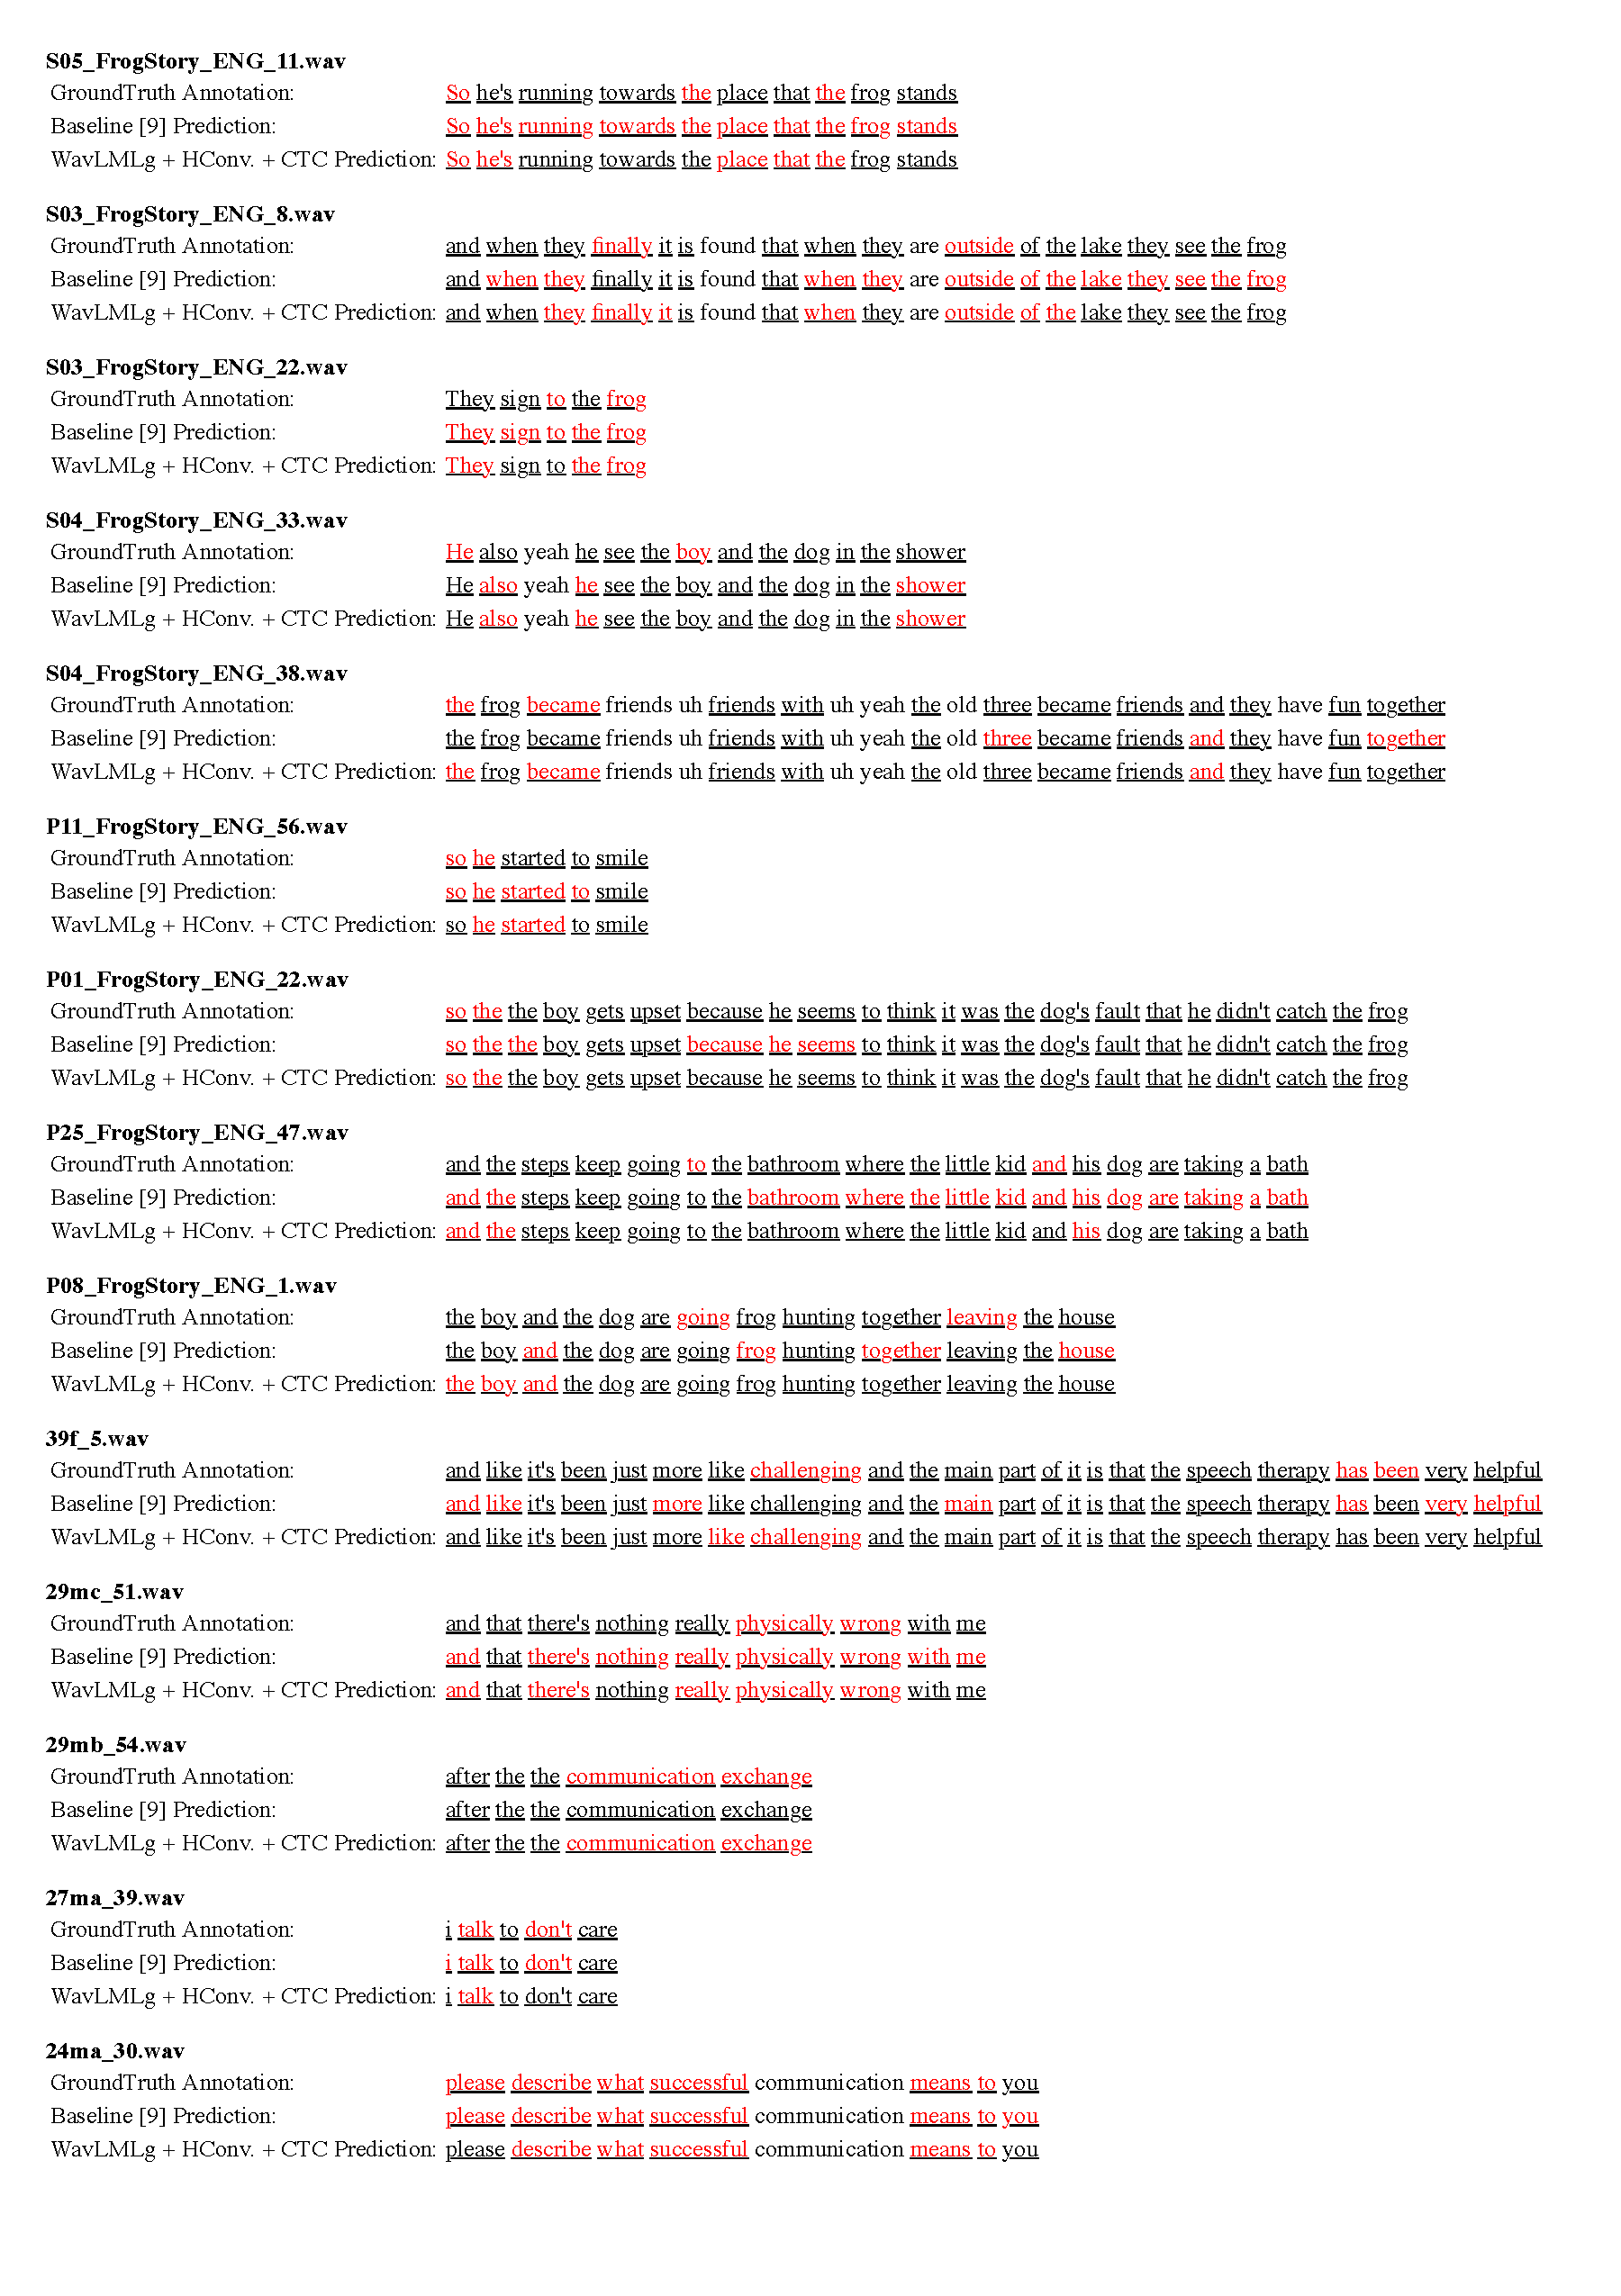
\includegraphics[width=0.9\textwidth,trim={0.2cm 26cm 6cm 0.9cm},clip]{figs/pdfs/qualitative_examples.pdf}
% 3 examples
% 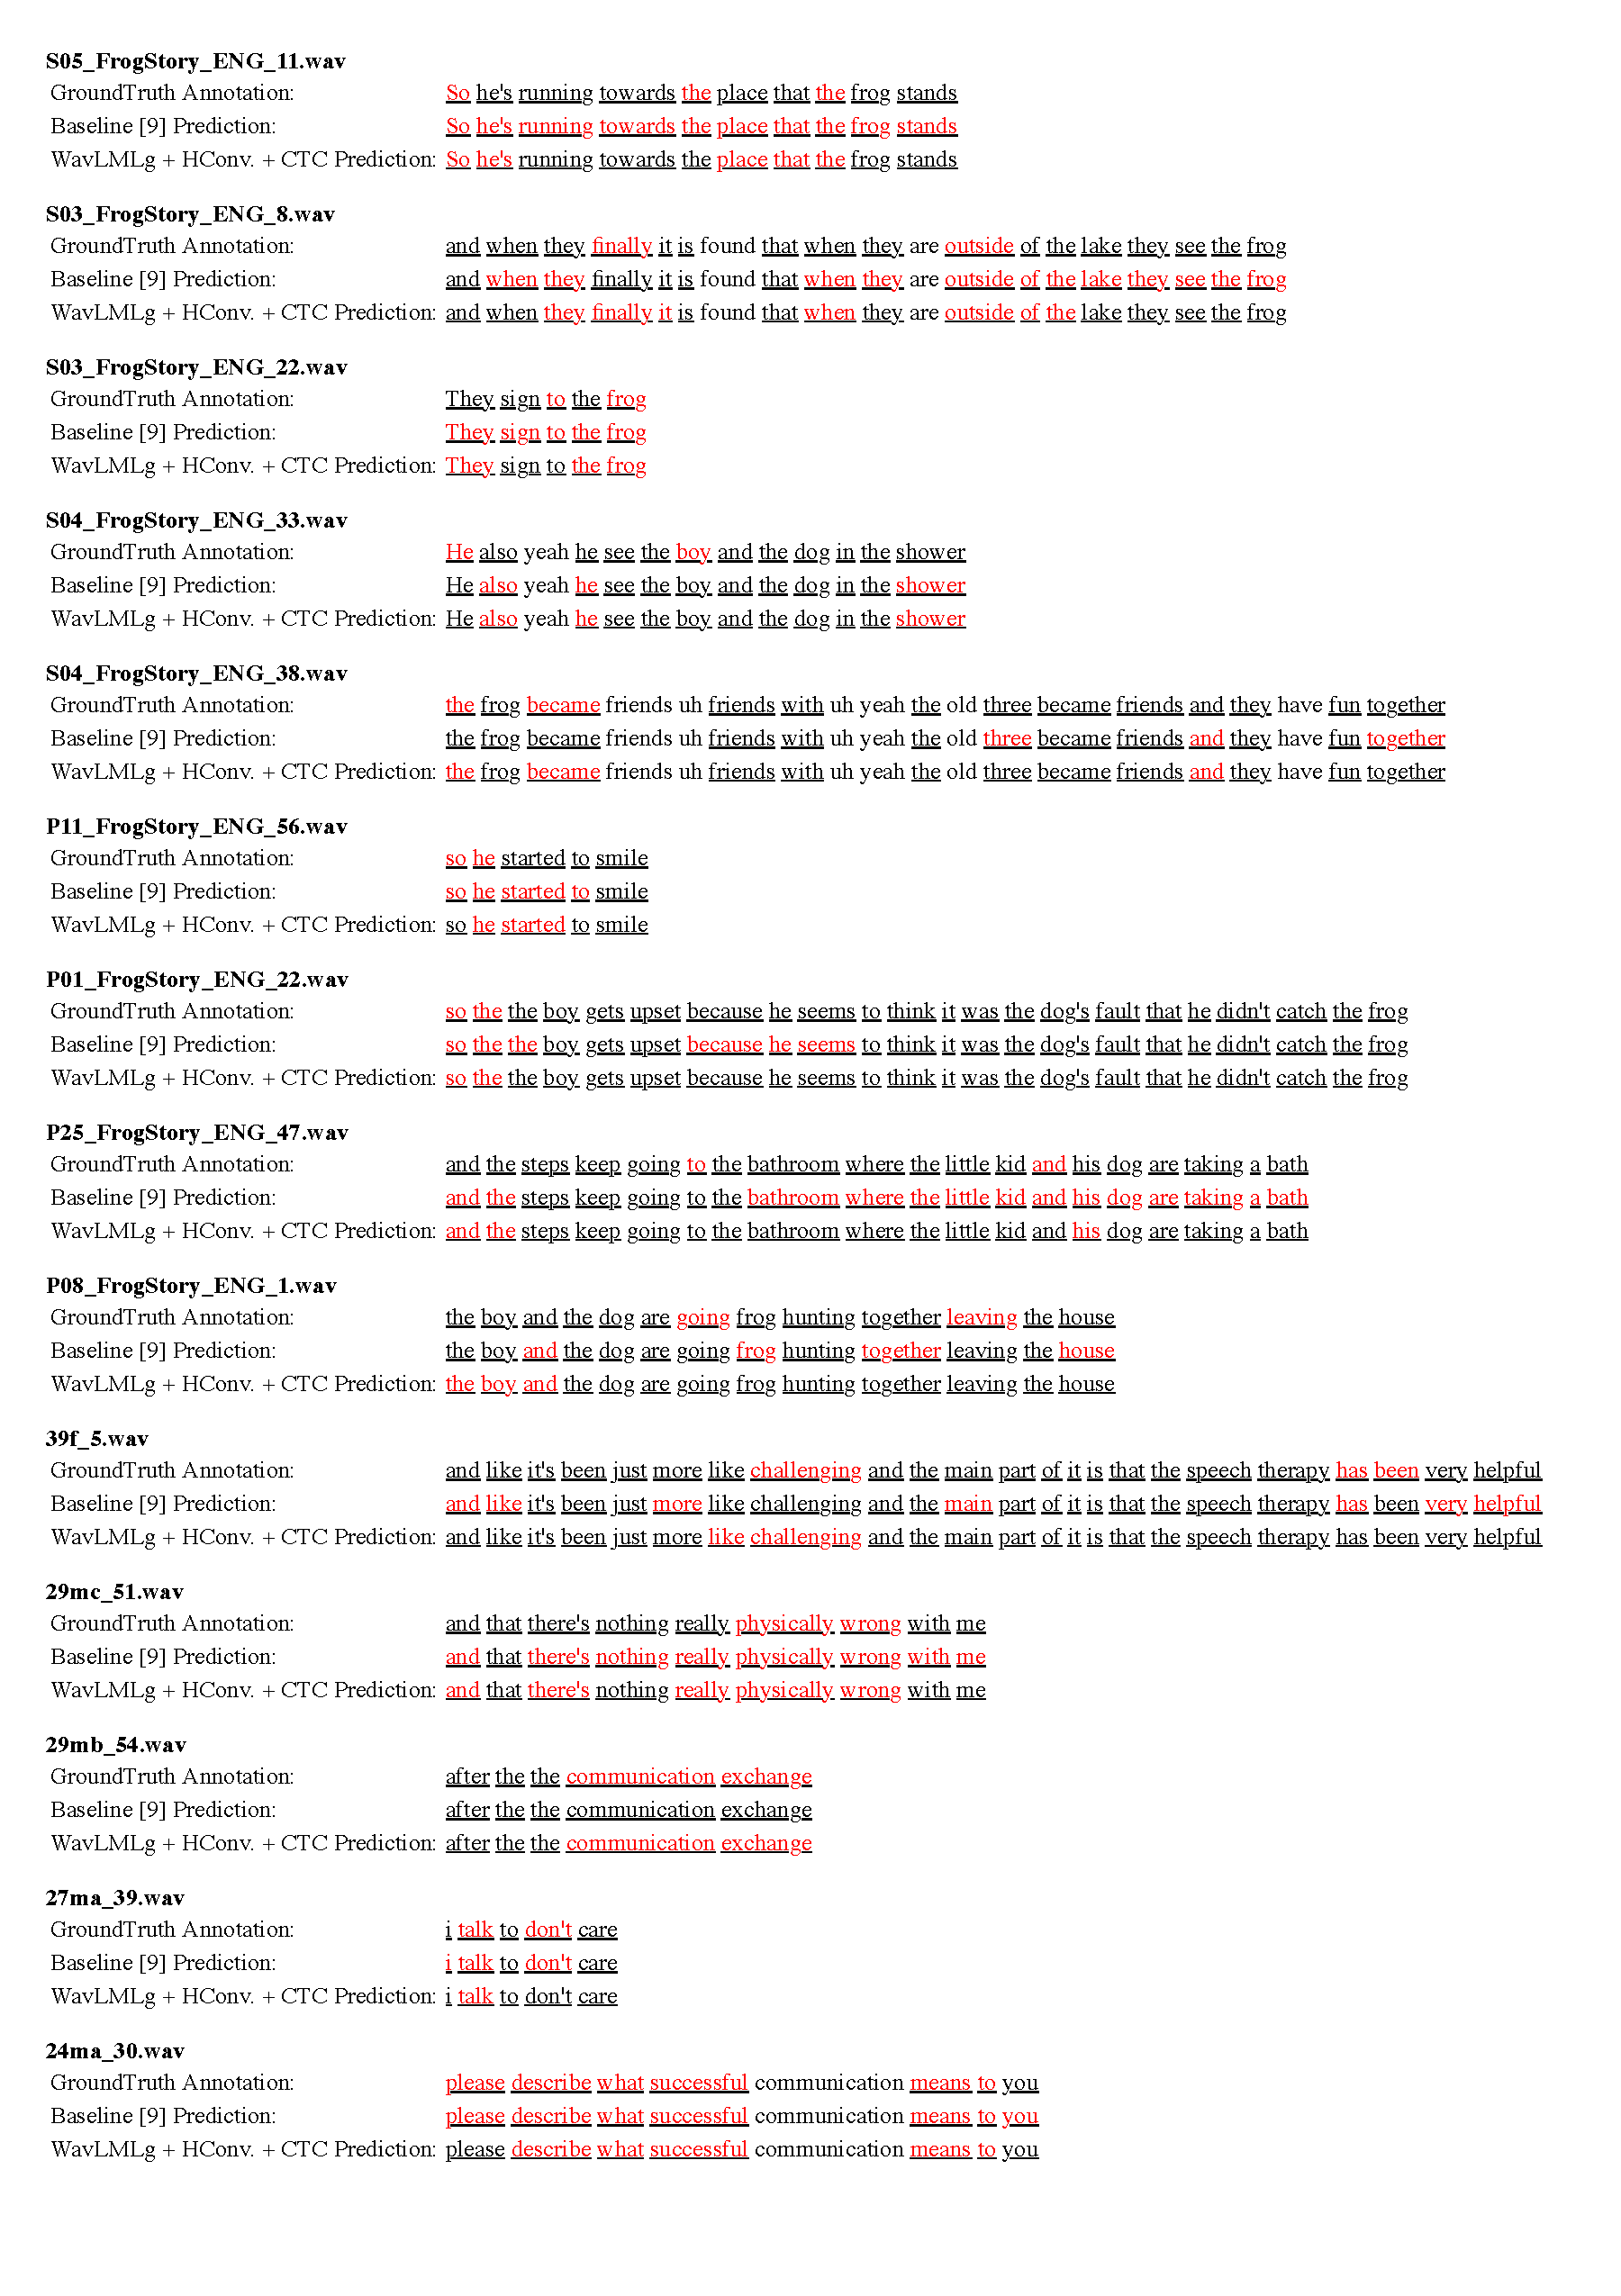
\includegraphics[width=0.9\textwidth,trim={0.2cm 34cm 6cm 0.9cm},clip]{figs/pdfs/qualitative_examples.pdf}
% 2 examples (title)
% 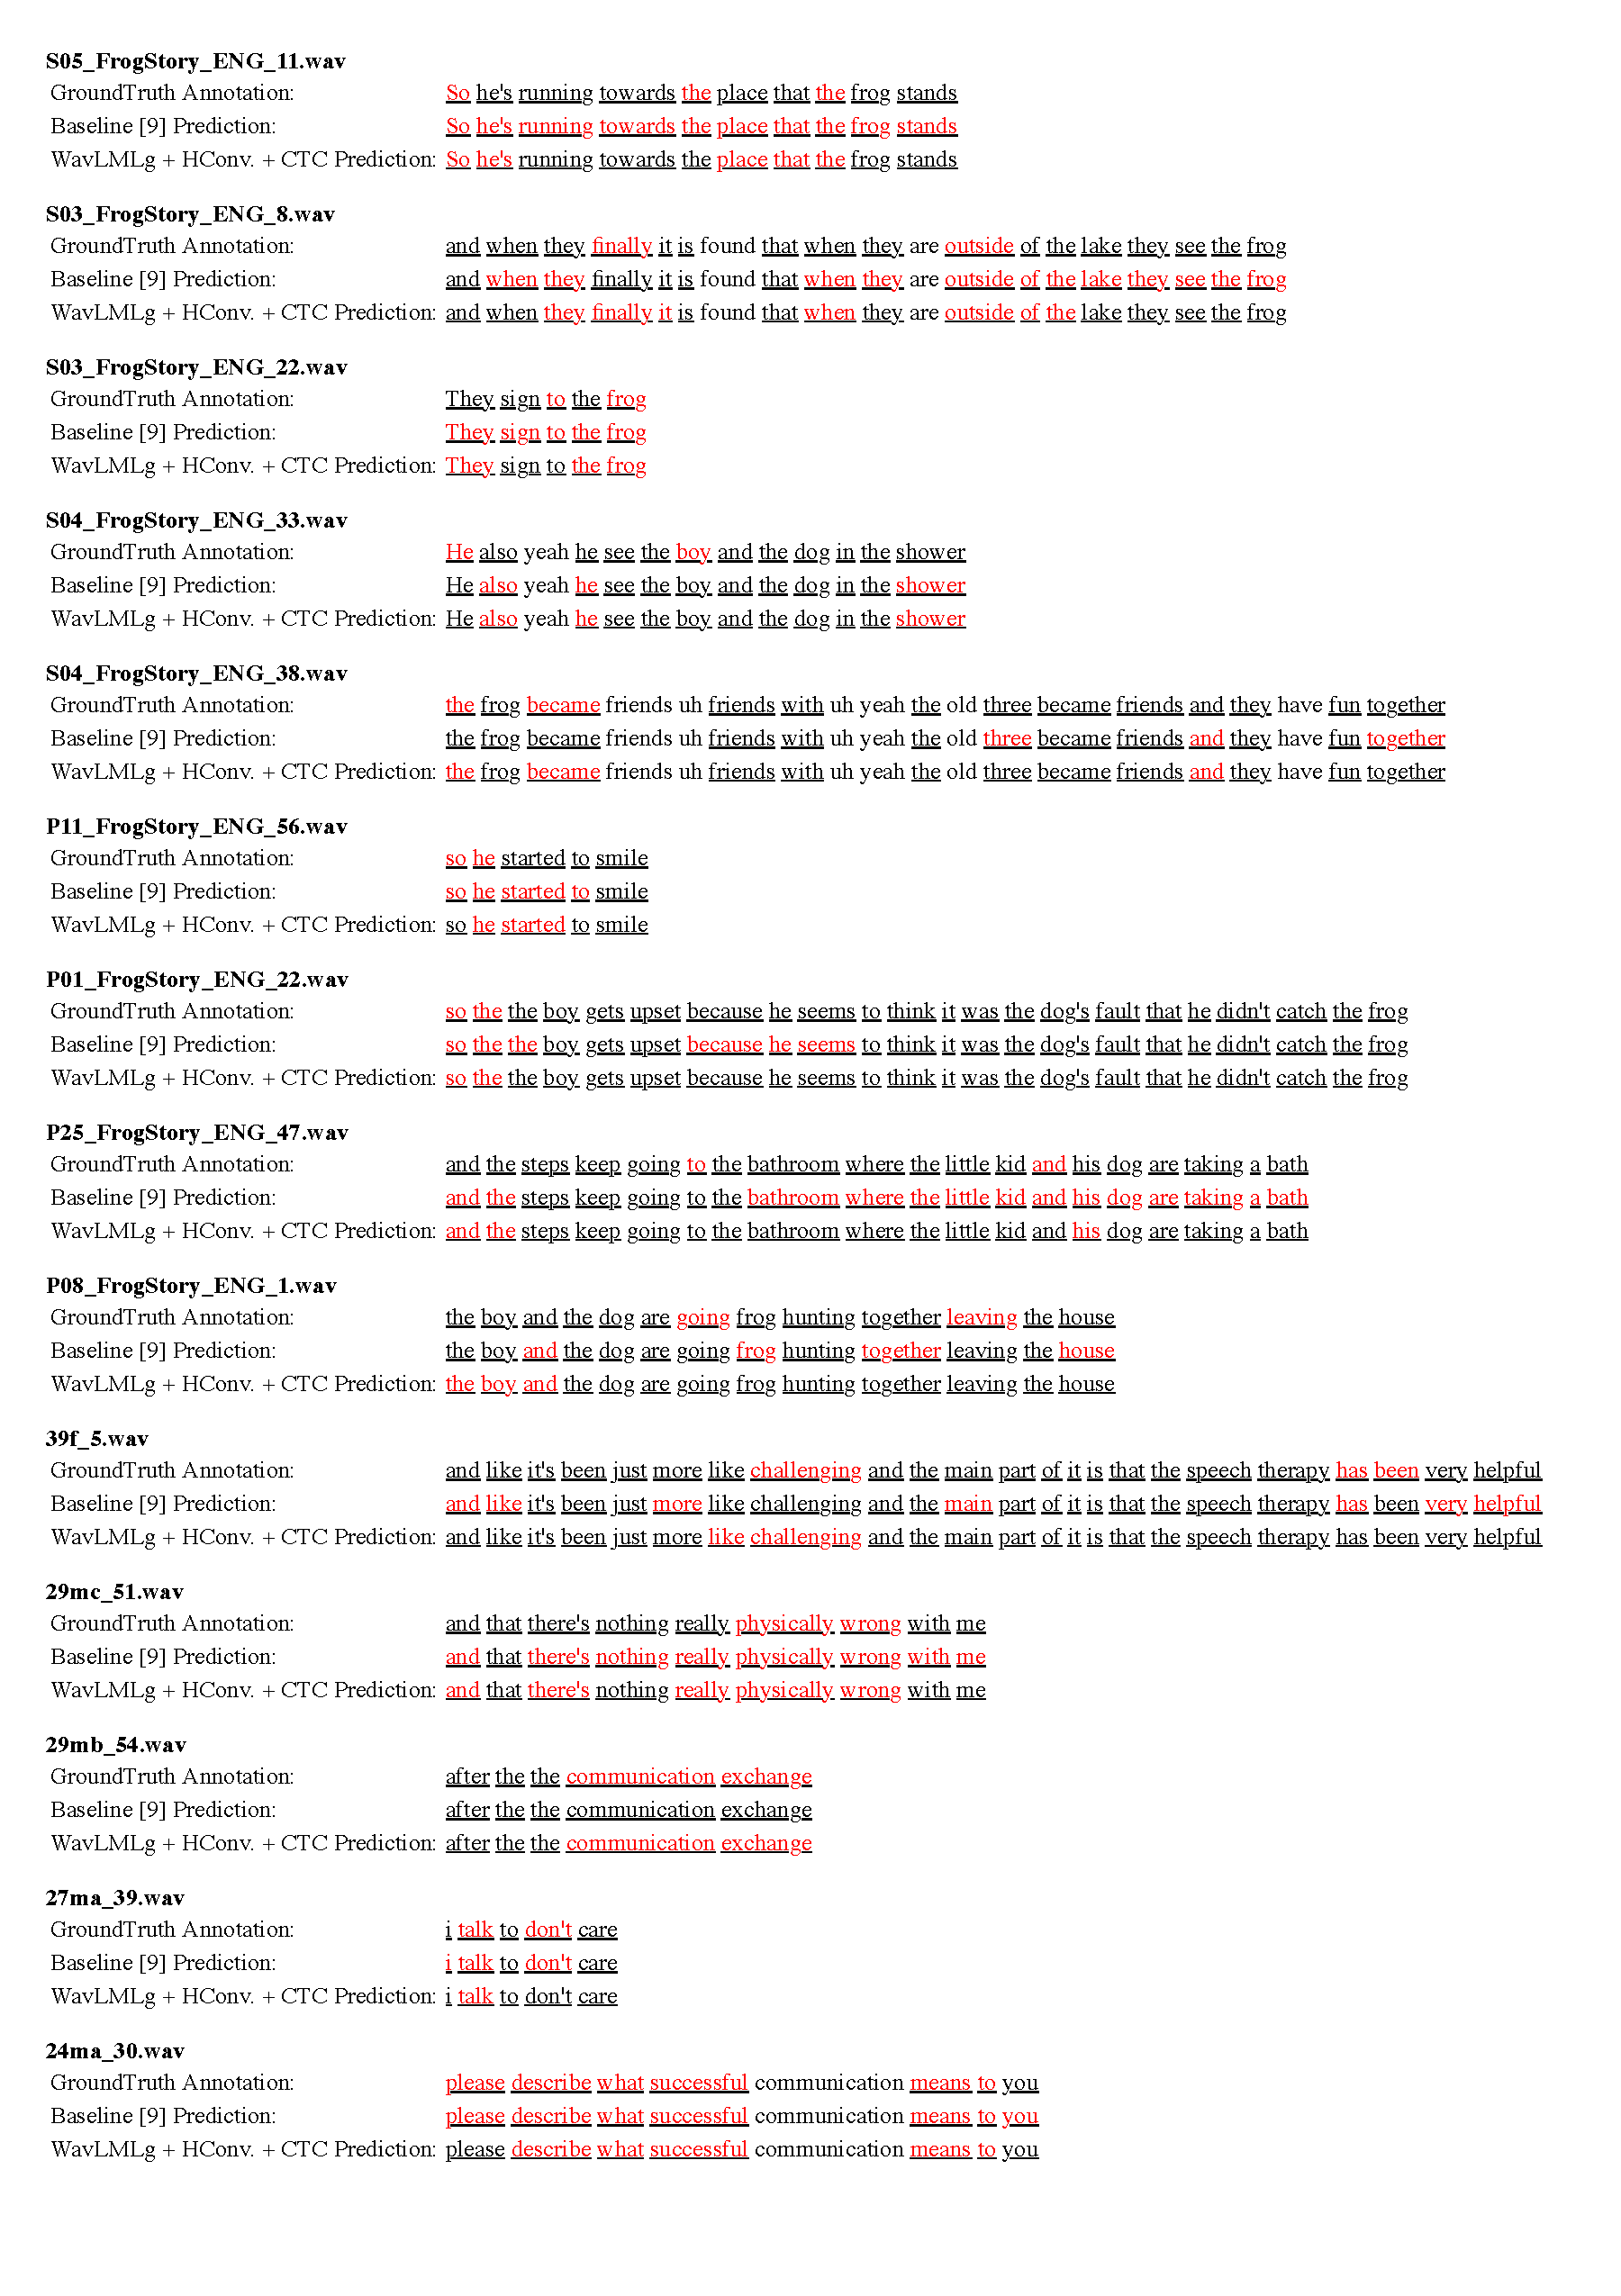
\includegraphics[width=0.9\textwidth,trim={0.2cm 37cm 6cm 0.9cm},clip]{figs/pdfs/qualitative_examples.pdf}
% 2 examples (no title)
% 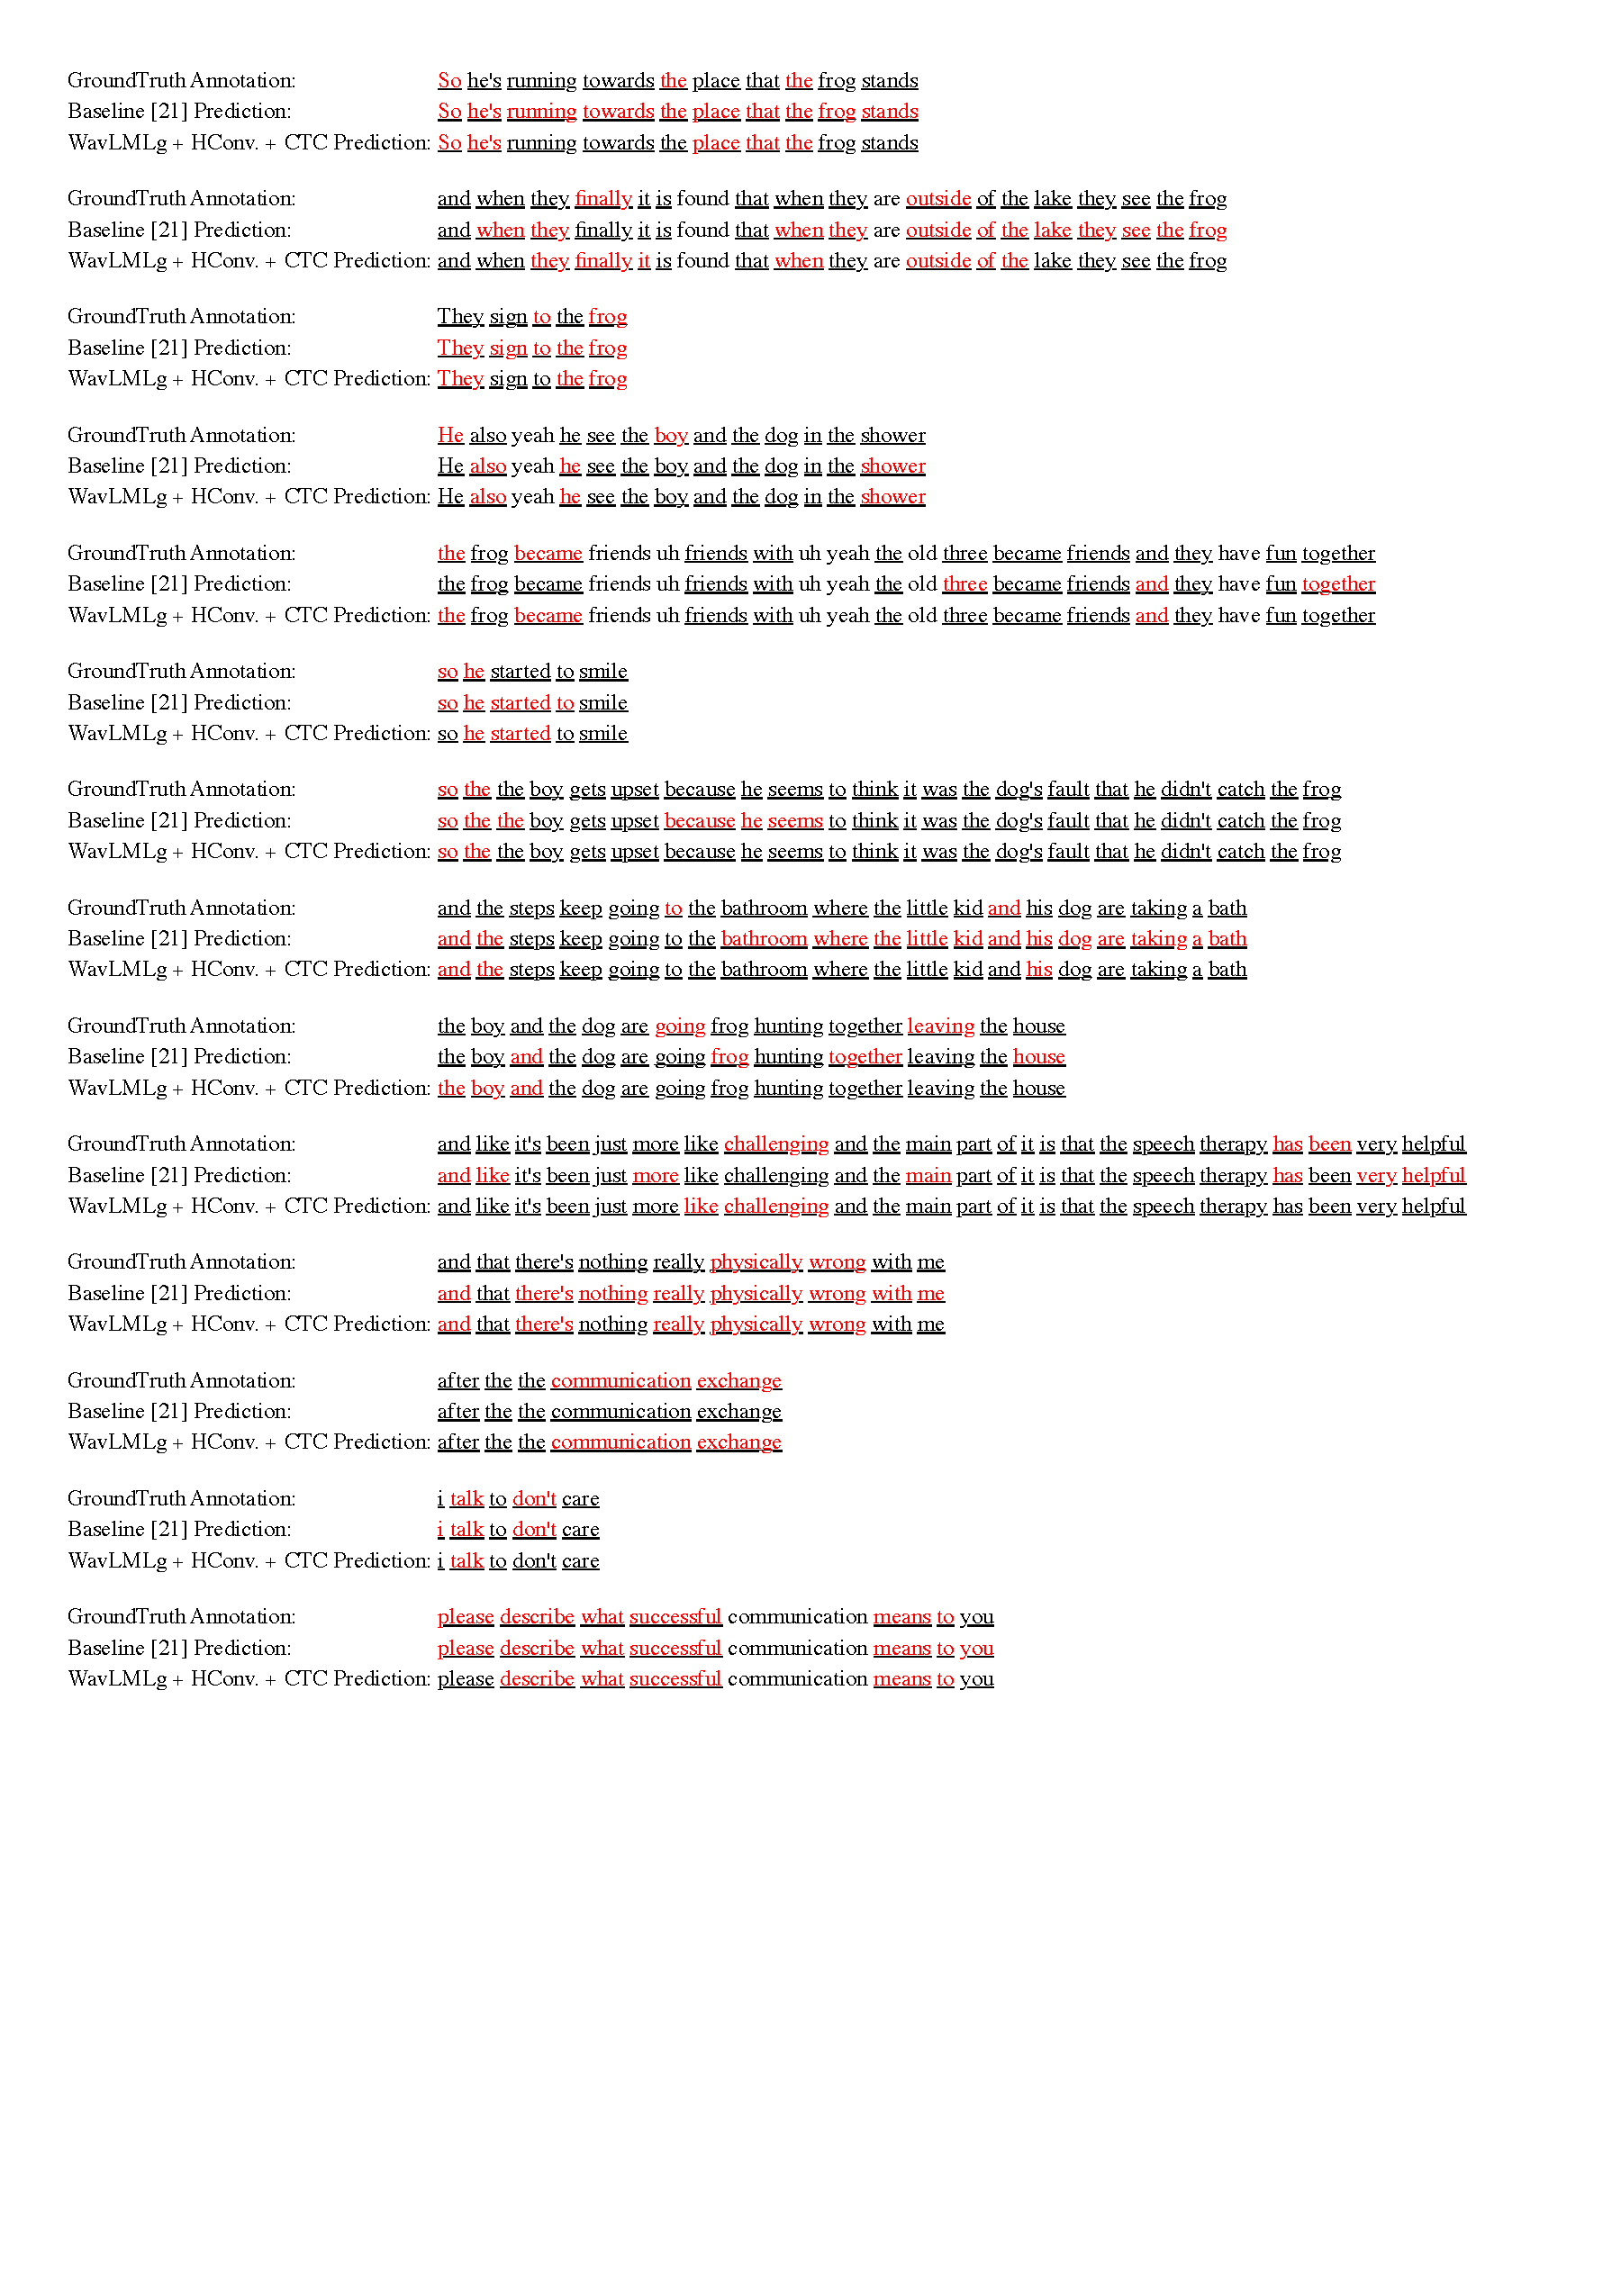
\includegraphics[width=0.9\textwidth,trim={0.2cm 38cm 7.4cm 0.9cm},clip]{figs/pdfs/qualitative_examples_noTitle.pdf}
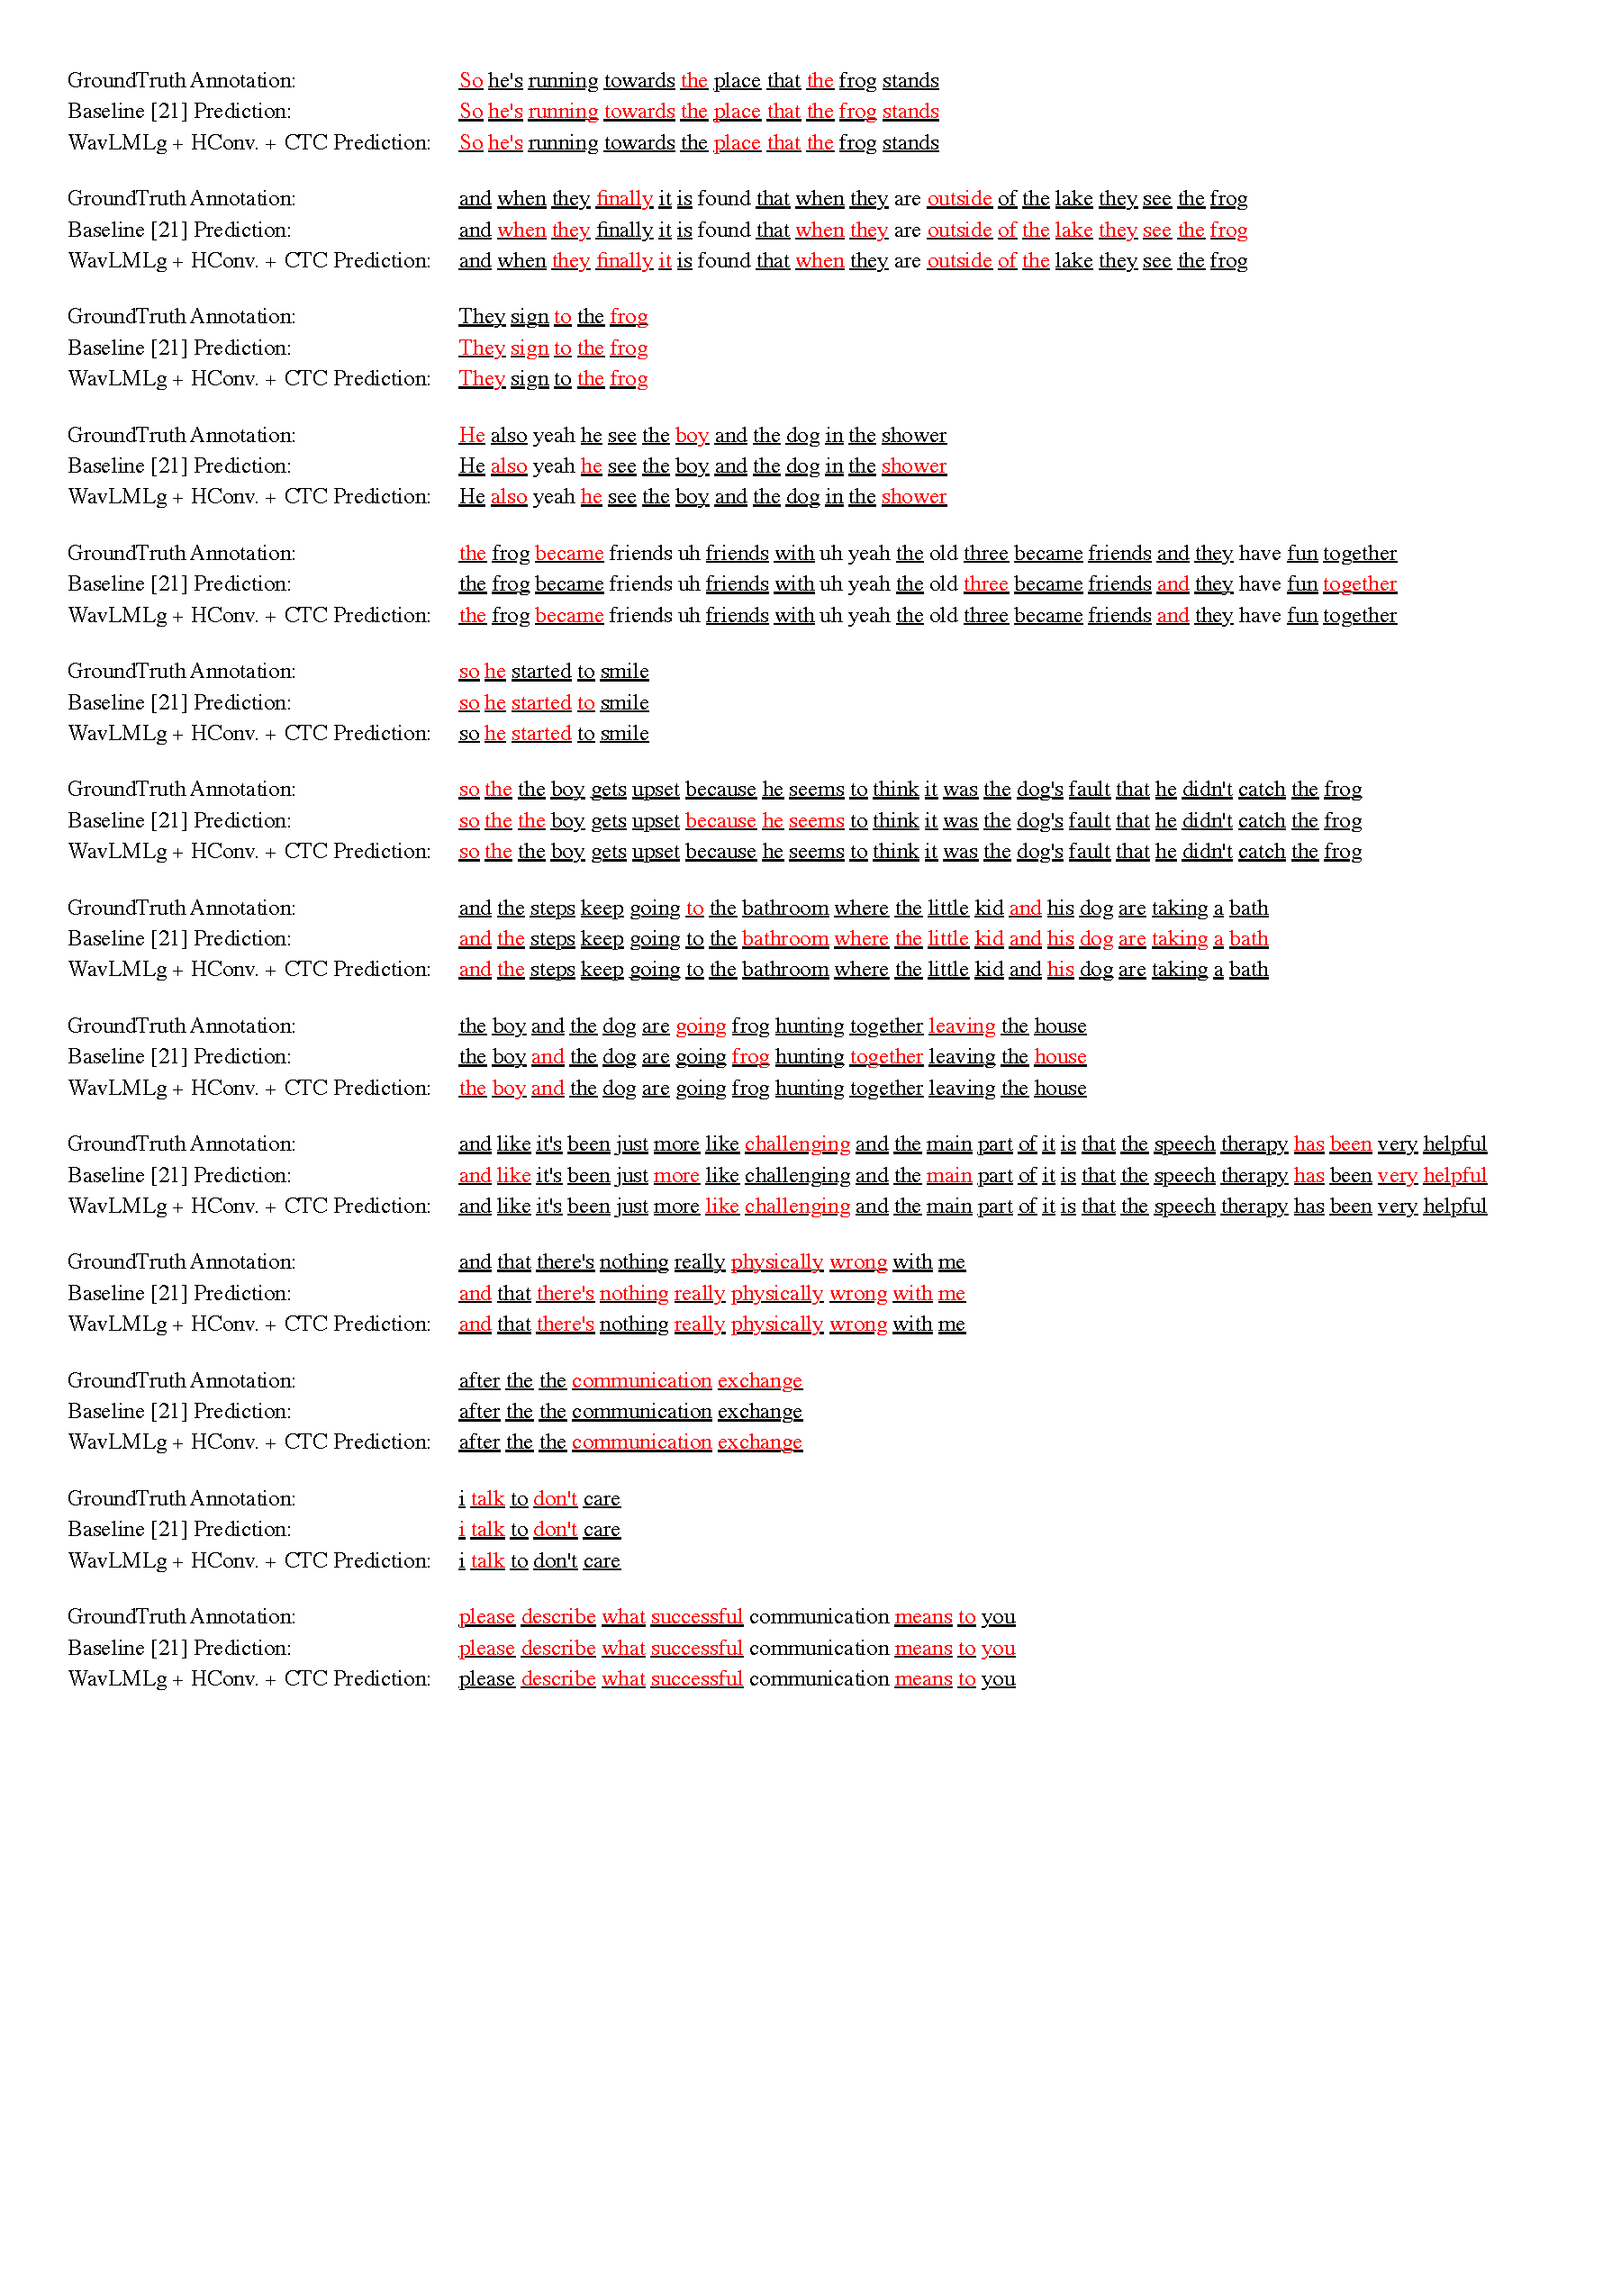
\includegraphics[width=0.9\textwidth,trim={0.2cm 38cm 7cm 0.9cm},clip]{figs/pdfs/qualitative_examples_noTitle_pad16.pdf}
\caption{Examples of our model and baseline model on word-level stuttering speech detection. Only the words with underscores are considered when evaluating. Words in red indicate that it is categorized as stuttered speech.
% \ian{will update the citation index for baseline later.} \david{maybe trim the number of examples here}
}
\label{fig:qualititave_examples}
\vspace{-10pt}
\end{figure*}